\paragraph{Measured reconstruction results.}
Table~\ref{tab:pidg-rendering} reports all 38 test images. Transferring appearance and refining boundary targets improves the connected model, while the unconstrained PIDG reconstruction remains stronger on recorded cameras. Larger output images use the same $320\times180$ training. These are held-image reconstruction scores, not forecasts of a new force.
\begin{center}
\captionof{table}{\textbf{PIDG Balls Reaction, matched image split.} Full-image / foreground PSNR (dB; higher is better), SSIM (higher) and AlexNet LPIPS (lower). The transferred model uses PIDG appearance initialization.}
\label{tab:pidg-rendering}
\begin{tabular}{llrrrr}
\toprule Output width & Method & PSNR & FG PSNR & SSIM & LPIPS \\
\midrule
320 & PIDG & 49.54 & 39.62 & 0.9987 & 0.0004 \\
320 & Ours: coarse appearance & 25.59 & 19.81 & 0.9210 & 0.0827 \\
320 & Ours: transferred appearance & 31.43 & 22.89 & 0.9710 & 0.0245 \\
\midrule
640 & PIDG & 34.48 & 25.28 & 0.9845 & 0.0086 \\
640 & Ours: coarse appearance & 25.50 & 19.28 & 0.9242 & 0.0823 \\
640 & Ours: transferred appearance & 29.86 & 20.83 & 0.9549 & 0.0442 \\
\midrule
1600 & PIDG & 31.64 & 22.41 & 0.9712 & 0.0323 \\
1600 & Ours: coarse appearance & 25.40 & 19.01 & 0.9335 & 0.0896 \\
1600 & Ours: transferred appearance & 28.68 & 19.35 & 0.9473 & 0.0662 \\
\bottomrule\end{tabular}\end{center}
\begin{center}\begin{minipage}{\textwidth}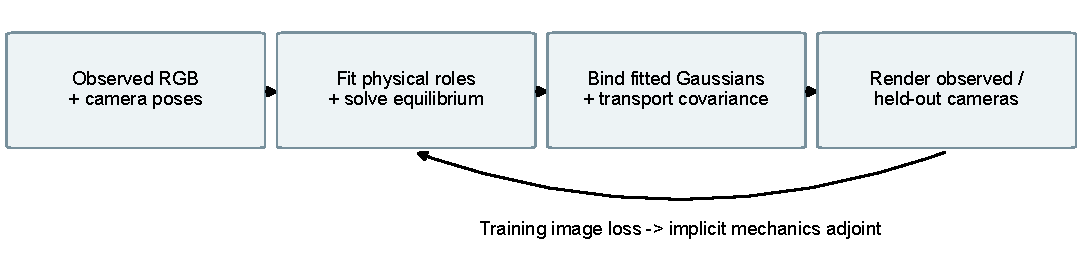
\includegraphics[width=\textwidth]{figures/pidg-rendering-loop.pdf}
\captionof{figure}{\textbf{Image loss reaches the physical state.} Boundary controls update solved equilibrium through an implicit adjoint. Appearance-only refinement then holds the selected mechanics fixed; query-time images use mechanics-transported Gaussians.}\end{minipage}\end{center}
\begin{center}\begin{minipage}{\textwidth}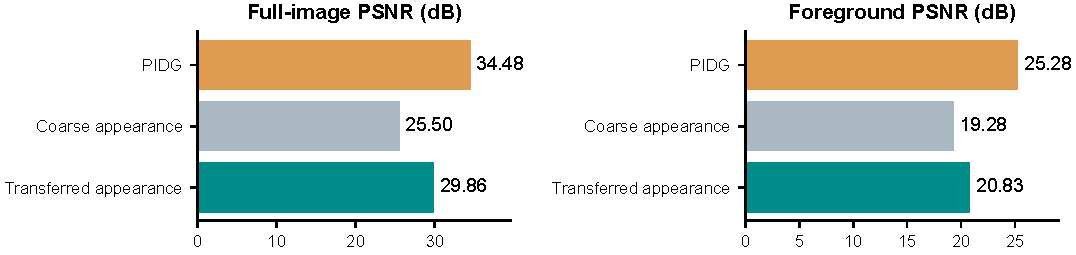
\includegraphics[width=\textwidth]{figures/pidg-rendering-metrics.pdf}
\captionof{figure}{\textbf{Aggregate recorded-camera reconstruction at width 640.} Foreground scores prevent the black background from dominating interpretation. Native PIDG remains ahead; the transferred mechanical renderer improves on its previous coarse initialization.}\end{minipage}\end{center}
\clearpage
\begin{center}\begin{minipage}{\textwidth}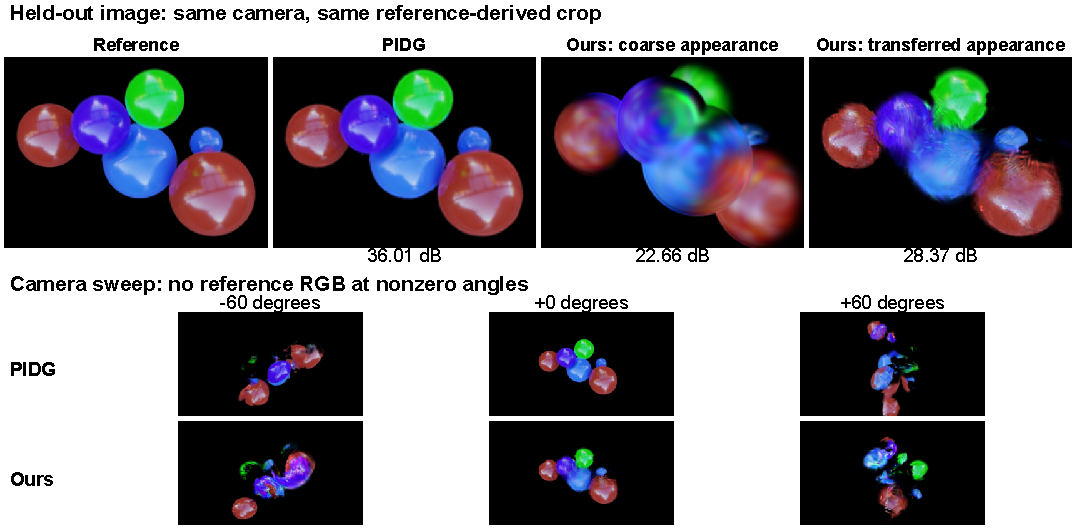
\includegraphics[width=\textwidth]{figures/pidg-rendering-comparison.pdf}
\captionof{figure}{\textbf{Appearance refinement and camera sweep.} The middle declared test time is fixed in advance. Top: identical reference-derived crop and per-frame full-image PSNR. Bottom: fixed camera offsets, with no reference RGB at nonzero angles. The spherical geometry prior contributes to coherence; these views do not prove hidden-surface accuracy or material identification.}\end{minipage}\end{center}
